\documentclass[12pt,a4paper]{article}
\usepackage[top=1.5cm, bottom=1.5cm, left=2.0cm, right=1.5cm] {geometry}
\usepackage{amsmath,amssymb,txfonts}
\usepackage{tkz-euclide}
\usepackage{setspace}
\usepackage{lastpage}

\usepackage{tikz,tkz-tab}
%\usepackage[solcolor]{ex_test}
%\usepackage[dethi]{ex_test} % Chỉ hiển thị đề thi
\usepackage[loigiai]{ex_test} % Hiển thị lời giải
%\usepackage[color]{ex_test} % Khoanh các đáp án
\everymath{\displaystyle}

\def\colorEX{\color{purple}}
%\def\colorEX{}%Không tô màu đáp án đúng trong tùy chọn loigiai
\renewtheorem{ex}{\color{violet}Câu}
\renewcommand{\FalseEX}{\stepcounter{dapan}{{\bf \textcolor{blue}{\Alph{dapan}.}}}}
\renewcommand{\TrueEX}{\stepcounter{dapan}{{\bf \textcolor{blue}{\Alph{dapan}.}}}}

%---------- Khai báo viết tắt, in đáp án
\newcommand{\hoac}[1]{ %hệ hoặc
    \left[\begin{aligned}#1\end{aligned}\right.}
\newcommand{\heva}[1]{ %hệ và
    \left\{\begin{aligned}#1\end{aligned}\right.}

%Tiêu đề
\newcommand{\tenso}{}
\newcommand{\tentruong}{}
\newcommand{\tenkythi}{ĐỀ ÔN TẬP}
\newcommand{\tenmonthi}{Môn thi: }
\newcommand{\thoigian}{}
\newcommand{\tieude}[1]{
   \begin{tabular}{cm{3cm}cm{3cm}cm{3cm}}
    {\bf \tenso} & & {\bf \tenkythi} \\
    {\bf \tentruong} & & {\bf \tenmonthi}\\
    && {\bf Thời gian: \bf \thoigian \, phút}\\
    && { \fbox{\bf Mã đề: #1}}
   \end{tabular}\\\\
    
   {Họ tên HS: \dotfill Số báo danh \dotfill}\\
}
\newcommand{\chantrang}[2]{\rfoot{Trang \thepage $-$ Mã đề #2}}
\pagestyle{fancy}
\fancyhf{}
\renewcommand{\headrulewidth}{0pt} 
\renewcommand{\footrulewidth}{0pt}
\usetikzlibrary{shapes.geometric,arrows,calc,intersections,angles,quotes,patterns,snakes,positioning}

\begin{document}
%Thiết lập giãn dọng 1.5cm 
%\setlength{\lineskip}{1.5em}
%Nội dung trắc nghiệm bắt đầu ở đây


\tieude{001}
\chantrang{\pageref{LastPage}}{001}
\setcounter{page}{1}
{\bf PHẦN I. Câu trắc nghiệm nhiều phương án lựa chọn.}
\setcounter{ex}{0}
\Opensolutionfile{ans}[ans/ans001-1]
\begin{ex}
 Cho hình chóp ${S.ABCD}$ có đáy là hình vuông tâm ${O}$. Gọi ${G,Q}$ lần lượt là trung điểm của ${SA,SD}$. Giao tuyến của hai mặt phẳng $(OGQ)$ và $(ABCD)$ là 
\begin{center}
 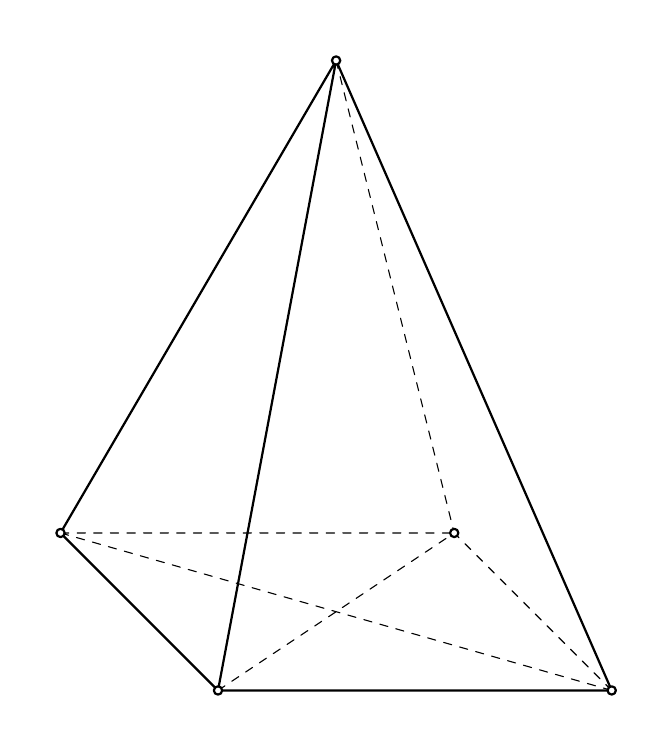
\begin{tikzpicture}[line join=round, line cap=round,thick]
\coordinate (A) at (0,0);
\coordinate (B) at (2,-2);
\coordinate (D) at (5,0);
\coordinate (C) at ($(B)+(D)-(A)$);
\coordinate (O) at ($(A)!0.5!(C)$);
\coordinate (S) at ($(O)+(0,7)$);
\draw(S)--(A) (S)--(B) (S)--(C) (A)--(B) (B)--(C);
\draw[dashed,thin](A)--(C) (A)--(D) (C)--(D) (S)--(D) (B)--(D);
\foreach \i/\g in {S/90,A/180,B/-90,C/-90,D/0}{\draw[fill=white](\i) circle (1.5pt) ($(\i)+(\g:3mm)$) node[scale=1]{};}
\end{tikzpicture}

\end{center}
\choice
{ đường thẳng qua ${O}$ và song song với ${AB}$ }
   { đường thẳng qua ${S}$ và song song với ${CD}$ }
     { đường thẳng qua ${S}$ và song song với ${GQ}$ }
    { \True đường thẳng qua ${O}$ và song song với ${BC}$ }
\loigiai{\begin{center}
 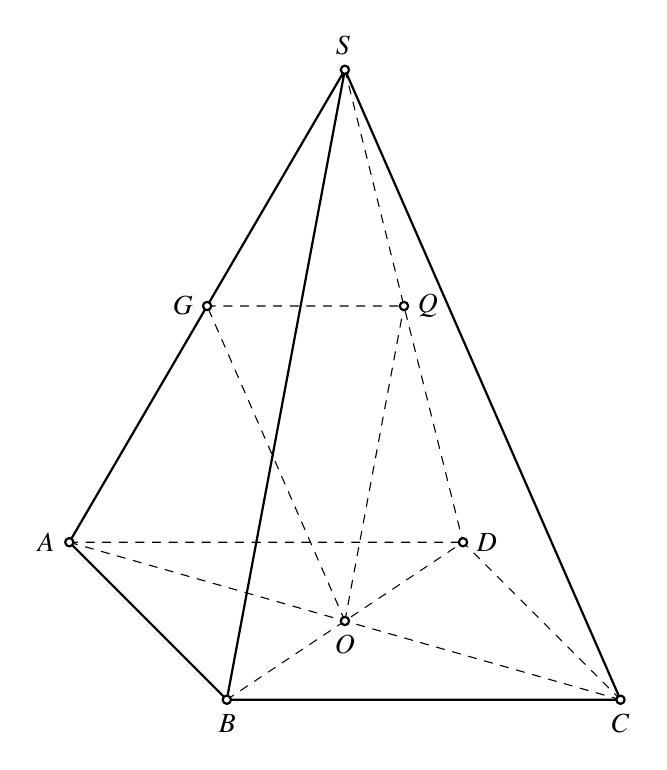
\begin{tikzpicture}[line join=round, line cap=round,thick]
		\coordinate (A) at (0,0);
		\coordinate (B) at (2,-2);
		\coordinate (D) at (5,0);
		\coordinate (C) at ($(B)+(D)-(A)$);
		\coordinate (O) at ($(A)!0.5!(C)$);
		\coordinate (S) at ($(O)+(0,7)$);
		\coordinate (G) at ($(S)!0.5!(A)$);
		\coordinate (Q) at ($(S)!0.5!(D)$);
		\draw(S)--(A) (S)--(B) (S)--(C) (A)--(B) (B)--(C) ;
		\draw[dashed,thin](A)--(C) (A)--(D) (C)--(D) (S)--(D) (B)--(D);
		\draw[dashed,thin](O)--(G) (O)--(Q) (G)--(Q);
		\foreach \i/\g in {S/90,A/180,B/-90,C/-90,D/0,O/-90,G/180,Q/0}{\draw[fill=white](\i) circle (1.5pt) ($(\i)+(\g:3mm)$) node[scale=1]{$\i$};}
		\end{tikzpicture}

\end{center}
 $\left\{ \begin{array}{l} 
			GQ\subset (OGQ) \\ 
			AD\subset (ABCD)\\ 
			GQ // AD 
			\end{array} \right.$$\Rightarrow (OGQ) \cap (ABCD)=Ox // AD //GQ //BC$. 
 }\end{ex}

\begin{ex}
 Cho hình chóp ${S.BCDE}$ có đáy là hình vuông tâm ${I}$. Gọi ${M,Q}$ lần lượt là trung điểm của ${SB,SE}$. Giao tuyến của hai mặt phẳng $(IMQ)$ và $(BCDE)$ là 
\begin{center}
 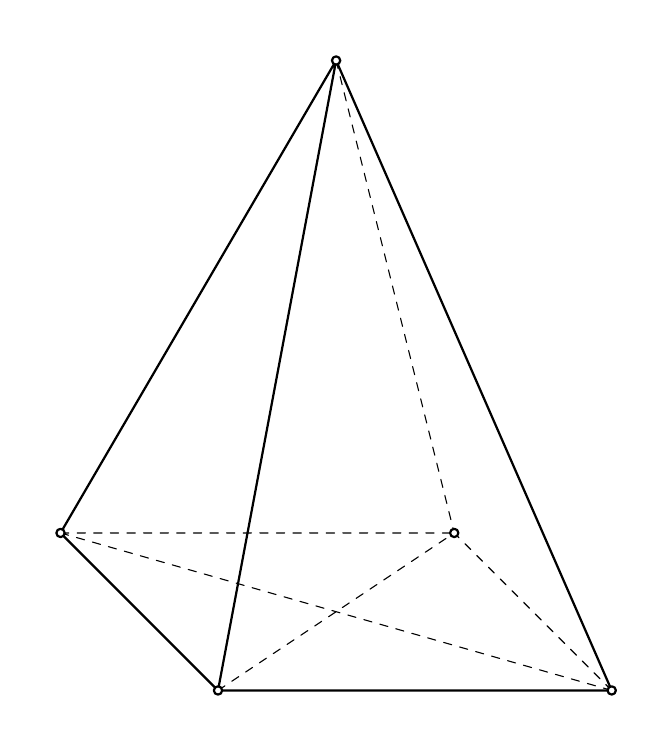
\begin{tikzpicture}[line join=round, line cap=round,thick]
\coordinate (B) at (0,0);
\coordinate (C) at (2,-2);
\coordinate (E) at (5,0);
\coordinate (D) at ($(C)+(E)-(B)$);
\coordinate (O) at ($(B)!0.5!(D)$);
\coordinate (S) at ($(O)+(0,7)$);
\draw(S)--(B) (S)--(C) (S)--(D) (B)--(C) (C)--(D);
\draw[dashed,thin](B)--(D) (B)--(E) (D)--(E) (S)--(E) (C)--(E);
\foreach \i/\g in {S/90,B/180,C/-90,D/-90,E/0}{\draw[fill=white](\i) circle (1.5pt) ($(\i)+(\g:3mm)$) node[scale=1]{};}
\end{tikzpicture}

\end{center}
\choice
{ đường thẳng qua ${S}$ và song song với ${MQ}$ }
   { đường thẳng qua ${I}$ và song song với ${BC}$ }
     { đường thẳng qua ${S}$ và song song với ${BC}$ }
    { \True đường thẳng qua ${I}$ và song song với ${BE}$ }
\loigiai{\begin{center}
 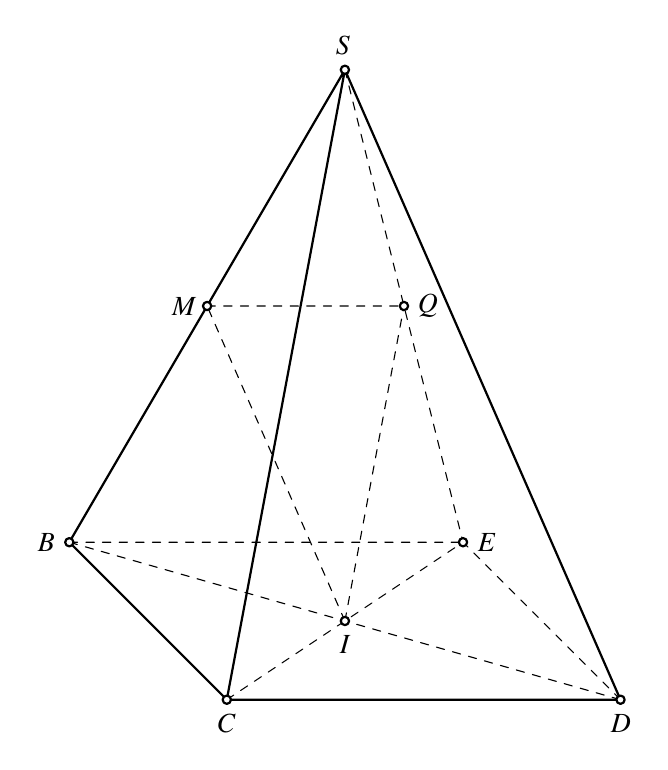
\begin{tikzpicture}[line join=round, line cap=round,thick]
		\coordinate (B) at (0,0);
		\coordinate (C) at (2,-2);
		\coordinate (E) at (5,0);
		\coordinate (D) at ($(C)+(E)-(B)$);
		\coordinate (I) at ($(B)!0.5!(D)$);
		\coordinate (S) at ($(I)+(0,7)$);
		\coordinate (M) at ($(S)!0.5!(B)$);
		\coordinate (Q) at ($(S)!0.5!(E)$);
		\draw(S)--(B) (S)--(C) (S)--(D) (B)--(C) (C)--(D) ;
		\draw[dashed,thin](B)--(D) (B)--(E) (D)--(E) (S)--(E) (C)--(E);
		\draw[dashed,thin](I)--(M) (I)--(Q) (M)--(Q);
		\foreach \i/\g in {S/90,B/180,C/-90,D/-90,E/0,I/-90,M/180,Q/0}{\draw[fill=white](\i) circle (1.5pt) ($(\i)+(\g:3mm)$) node[scale=1]{$\i$};}
		\end{tikzpicture}

\end{center}
 $\left\{ \begin{array}{l} 
			MQ\subset (IMQ) \\ 
			BE\subset (BCDE)\\ 
			MQ // BE 
			\end{array} \right.$$\Rightarrow (IMQ) \cap (BCDE)=Ix // BE //MQ //CD$. 
 }\end{ex}

\begin{ex}
 Cho hình chóp ${S.CDEF}$ có đáy là hình chữ nhật tâm ${O}$. Gọi ${P,H}$ lần lượt là trung điểm của ${SC,SD}$. Giao tuyến của hai mặt phẳng $(OPH)$ và $(CDEF)$ là 
\begin{center}
 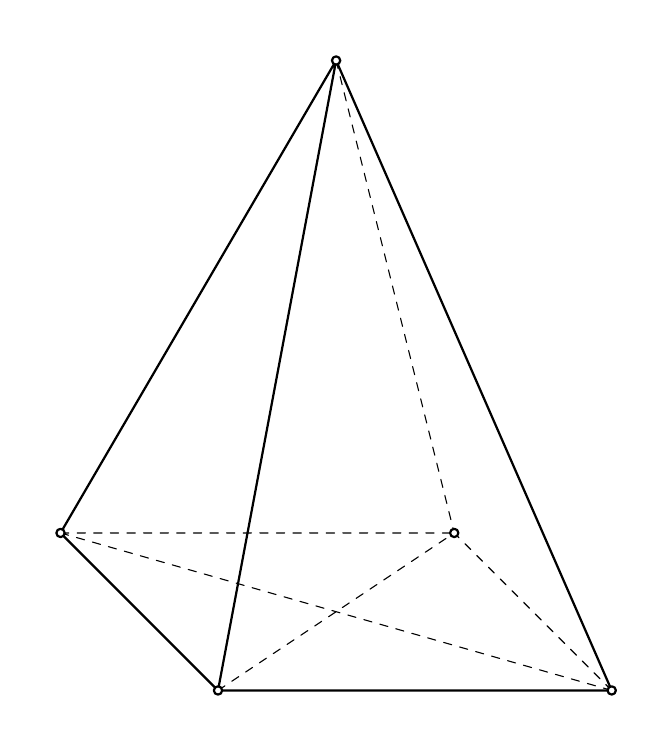
\begin{tikzpicture}[line join=round, line cap=round,thick]
\coordinate (C) at (0,0);
\coordinate (D) at (2,-2);
\coordinate (F) at (5,0);
\coordinate (E) at ($(D)+(F)-(C)$);
\coordinate (O) at ($(C)!0.5!(E)$);
\coordinate (S) at ($(O)+(0,7)$);
\draw(S)--(C) (S)--(D) (S)--(E) (C)--(D) (D)--(E);
\draw[dashed,thin](C)--(E) (C)--(F) (E)--(F) (S)--(F) (D)--(F);
\foreach \i/\g in {S/90,C/180,D/-90,E/-90,F/0}{\draw[fill=white](\i) circle (1.5pt) ($(\i)+(\g:3mm)$) node[scale=1]{};}
\end{tikzpicture}

\end{center}
\choice
{ \True đường thẳng qua ${O}$ và song song với ${PH}$ }
   { đường thẳng qua ${S}$ và song song với ${CD}$ }
     { đường thẳng qua ${S}$ và song song với ${CF}$ }
    { đường thẳng qua ${O}$ và song song với ${DE}$ }
\loigiai{\begin{center}
 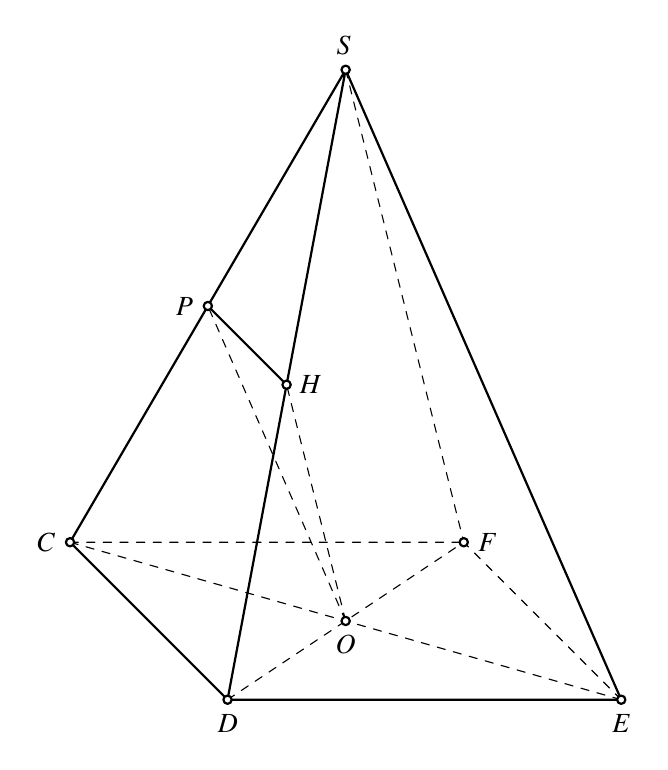
\begin{tikzpicture}[line join=round, line cap=round,thick]
		\coordinate (C) at (0,0);
		\coordinate (D) at (2,-2);
		\coordinate (F) at (5,0);
		\coordinate (E) at ($(D)+(F)-(C)$);
		\coordinate (O) at ($(C)!0.5!(E)$);
		\coordinate (S) at ($(O)+(0,7)$);
		\coordinate (P) at ($(S)!0.5!(C)$);
		\coordinate (H) at ($(S)!0.5!(D)$);
		\draw(S)--(C) (S)--(D) (S)--(E) (C)--(D) (D)--(E) (P)--(H);
		\draw[dashed,thin](C)--(E) (C)--(F) (E)--(F) (S)--(F) (D)--(F);
		\draw[dashed,thin](O)--(P) (O)--(H) ;
		\foreach \i/\g in {S/90,C/180,D/-90,E/-90,F/0,O/-90,P/180,H/0}{\draw[fill=white](\i) circle (1.5pt) ($(\i)+(\g:3mm)$) node[scale=1]{$\i$};}
		\end{tikzpicture}

\end{center}
 $\left\{ \begin{array}{l} 
			PH\subset (OPH) \\ 
			CD\subset (CDEF)\\ 
			PH // CD 
			\end{array} \right.$$\Rightarrow (OPH) \cap (CDEF)=Ox // CD //PH //EF$. 
 }\end{ex}

\Closesolutionfile{ans}

 \begin{center}
-----HẾT-----
\end{center}

 %\newpage 
%\begin{center}
%{\bf BẢNG ĐÁP ÁN MÃ ĐỀ 1 }
%\end{center}
%{\bf Phần 1 }
% \inputansbox{6}{ans001-1}



\end{document}